\documentclass[12pt,titlepage]{article}

\usepackage{amsmath,graphicx,a4wide,fontspec,hyperref}
\usepackage[ngerman]{babel}
\setmainfont{Helvetica Neue}
\setmonofont{Menlo Regular}

\begin{document}

\title{Miniprojekt: \\ Minimax-Maschine \\ Dokumentation}
\author{Clemens Pollak, Robin Thrift, Max Boll}
\date{Hardware Projekt 2014 \\ 14.11.2014}
\maketitle

\tableofcontents

\newpage

\section{Einleitung} 
Unser gew{\"a}hltes Thema befasst sich mit der Minimax-Maschine und der Realisierung von Algorithmen auf dieser. Es soll im Rahmen des Hardware-Praktikums bearbeitet werden und ist uns aus der Veranstaltung "'Grundlagen der Rechnerarchitektur"' bereits grundlegend bekannt.\\ Dieses Dokument soll eine Dokumentation darstellen, die dem besseren Verst{\"a}ndnis unserer Implementierung dienen soll.


\section{Aufgabenstellung}
Nach unserer Auffassung ist das Ziel dieser Aufgabenstellung ein Algorithmus, welcher auf der Minimax-Maschine zu implementieren ist und eine sogenannte Paketanalyse betreibt. Dieser "'Paketanalyse"'-Algorithmus befasst sich mit den Datenpaketen, die im Speicher der Minimax-Maschine abgelegt sind.\\ Ein Datenpaket beginnt immer mit der Folge "'1110"' und besteht aus einem
Kopf mit einer L{\"a}nge von 80 Bits und einem Datenteil mit variabler L{\"a}nge. Der Kopf enth{\"a}lt die Kanalnummer zwischen der 32. und 47. Bitstelle. Zu einem Kanal k{\"o}nnen ein oder mehrere Pakete geh{\"o}ren, die dieselbe Kanalnummer haben.
Die Anzahl der Bits, die überprüft werden müssen, wird als bekannt vorausgesetzt und in ein entsprechendes Register vorgeladen.\\
Nun soll der Algorithmus eine Datentabelle anlegen, welche sich au{\ss}erhalb der Speicherfelder der einzelnen Pakete befindet. Diese Datentabelle soll den Kanalnummern die L{\"a}ngen der jeweiligen Datenteile aller Pakete zuordenen, um dann später exportiert zu werden. Diese Aufgabenstellung soll mit dem Minimax-Simulator simuliert und getestet werden. Die Maschine kann durch vorgegebene Bauteile erweitert werden, was sich aber auf die Bewertung auswirkt. Der Algorithmus wird in Form der sogenannten Steuertabelle implementiert und soll außerdem als Flussdiagramm abgegeben werden.

\newpage

\section{Ist-Analyse der Basis-Maschine}

Die Minimax-Maschine ist ein minimales Rechensystem, das aus einfachen Registern (Basis: \texttt{ACCU}, \texttt{PC}, \texttt{IR}, \texttt{MDR}, \texttt{MAR};
weitere k{\"o}nnen hinzugef{\"u}gt werden), einer arithmetisch-logischen Einheit (ALU) und einem Hauptspeicher (HS) aufgebaut
ist und durch ein Mikroprogramm gesteuert wird. Jedes dieser Register hat als Eingang mindestens die ALU und zusätzlich einen Eingang, der den Schreibzugriff regelt.\\
\begin{enumerate}
\item \texttt{ACCU}: Abk{\"u}rzung f{\"u}r "'Accumulator"', ein Zwischenspeicher, um mit \texttt{MDR} Operationen durchführen zu k{\"o}nnen.
\item \texttt{PC}: Abk{\"u}rzung f{\"u}r "'program counter"', enthält den Programmzähler, welcher den nächsten Befehl beeinflusst
\item \texttt{IR}: Abk{\"u}rzung f{\"u}r "'instruction register"', enthält Opcode(8 Bit) und Adressteil(24 bit).
\item \texttt{MDR}: Abk{\"u}rzung f{\"u}r "'memory data register"', enthält je nach Einstellung des Multiplexers texttt{MDR.Sel}, verschiedene Daten, entweder aus dem Hauptspeicher oder aus der \texttt{ALU}.
\item \texttt{MAR}: Abk{\"u}rzung f{\"u}r "'memory adress register"', enth{\"a}lt die Speicheradresse, an der aus dem Hauptspeicher Daten geladen oder geschrieben werden sollen.
\item \texttt{HS}: Abk{\"u}rzung f{\"u}r "'Hauptspeicher"', er wird mit 24-Bit durch \texttt{MAR} adressiert und gibt eine 32-Bit Zahl zur{\"u}ck. Auf dieselbe Art funktioniert das Schreiben einer 32-Bit Zahl nat{\"u}rlich auch.
\end{enumerate}

\leavevmode \\

\begin{enumerate}
\item \texttt{ADD}: Addiert ALU-Eingang A und ALU-Eingang B
\item \texttt{SUB.B}: Subtrahiert ALU-Eingang A von ALU-Eingang B
\item \texttt{TRANS.A}: Schaltet den ALU-Eingang A durch
\item \texttt{TRANS.B}: Schaltet den ALU-Eingang B durch
\end{enumerate}

\leavevmode \\
Dabei sind die m{\"o}glichen Operationen auf die in der ALU implementieren
Operationen beschr{\"a}nkt (Basis: \texttt{ADD}, \texttt{SUB.B}, \texttt{TRANS.A}, \texttt{TRANS.B}). Die ALU kannn mit weiteren Operationen,
wie z.B. dem bitweisen UND, erg{\"a}nzt werden.\\
Um eine Operation auszuf{\"u}hren, m{\"u}ssen {\"u}ber die Multiplexer \texttt{ALUSel.A} und \texttt{AluSel.B} zwei Operanden ausgew{\"a}hlt werden
und der ALU muss {\"u}ber die \texttt{ALU Ctrl}-Leitung der Code f{\"u}r die Operation {\"u}bergeben werden. An den Multiplexern liegen sowohl
Konstanten als auch die Register an, welche zur ALU durchgeschaltet werden k{\"o}nnen. Das Ergebnis der Operation kann
entweder in einem Register oder (über MDR) im HS (Adresse im Register \texttt{MAR}) gespeichert werden. Zus{\"a}tzlich k{\"o}nnen sog. Flags (Basis nur ein Flag \texttt{ALU RESULT == 0})
gesetzt werden, welche zur{\"u}ck zur Control Unit (CU) geleitet werden, um z.B. bedingte Spr{\"u}nge auszuf{\"u}hren.
Abbildung 1 zeigt die uns vorliegende Basismaschine.

\leavevmode \\
Die uns vorliegende Minimax-Maschine arbeitet mit 32-Bit und speichert Werte mit 32-Bit in den Registern und im HS (\dq Little Endian\dq ).
Alle ALU-Operationen werden folglich mit 32-Bit ausgef{\"u}hrt. Dies stellt sich jedoch f{\"u}r unsere Aufgabe als
Hindernis dar, da wir die Daten bitweise untersuchen m{\"u}ssen, Daten aus dem HS und den Registern jedoch nur als
32-Bit Zahlen auslesen k{\"o}nnen und nicht als einzelne Bits.
Daher wird die Basismaschine um einige Konstanten, Operationen und Register erweitert werden müssen, welche im "'Implementierungskonzept"' n{\"a}her
aufgeführt sind. Abbildung 6 zeigt den Aufbau der erweiterten Maschine.

\newpage

\section{Finale Implementierung}
Wir haben das Hauptproblem in einige Teilprobleme aufgeteilt:
\begin{enumerate}
\item Das sequenzielle Auslesen des Hauptspeichers
\item Die Analyse der Daten
    \begin{enumerate}
    \item Das Erkennen der Startsequenz eines neuen Pakets
    \item Das Auslesen der Kanalnummer
    \end{enumerate}
\item Das Speichern der geforderten Daten im HS
\end{enumerate}

\subsection{Auslesen aus dem Hauptspeicher}
Damit die Maschine korrekt terminiert, muss zun{"a}chst die gegebene Gesamtlänge der zu analysierenden Daten überprüft werden. Sie liegt im Register \texttt{COUNT}.
Der Algorithmus l{"a}d eine neue 32-Bit-Folge und dekrementiert das Register \texttt{COUNT} danach um 32. Wenn das Register Null enth{"a}lt, terminiert damit das gesamte Programm. Ansonsten werden die Daten analysiert.\\
Die Überprüfung wird nach jeder Analyse wiederholt.

 

\subsection{Analyse der Daten}
Die Analyse der Daten kann als einfacher endlicher Automat mit 2 Zuständen betrachtet werden (0, 1). Im ersten Zustand (0)
wurde noch kein Paket gefunden und es wird mithilfe einer Bitmaske ($1111_{2} = 15_{10}$) nach der Anfangssequenz gesucht. 
Zunächst wird ab dem \dq Least Significant Bit\dq gesucht. Wird dort das Muster nicht gefunden, wird die Bitmaske (und die
Subtraktionszahl) so lange nach links \dq geschiftet\dq bis die Startsequenz gefunden wurde, oder
alle möglichen Positionen des Muster erschöpft wurden (Zahl ist Datenteil).
Wenn die Startsequenz gefunden wurde, wird der Zustand verändert (zu 1) und es wird auf die nächste Zahl aus dem HS gewartet. 
In der nächsten Zahl aus dem HS befindet sich die Kanalnummer. Diese wird mit einer weiteren Bitmaske ausgelesen
und im Register \texttt{CHNL} abgelegt.
Wurde sowohl ein Paketanfang als auch eine Kanalnummer gefunden, so wird nun die Länge des Datenfeldes gezählt und im Register \texttt{DATAC} gespeichert, bis erneut die Startsequenz gefunden wird.
Wurde eine neue Startsequenz gefunden, so wird von der Länge des Daten 16 abgezogen (16 Bits Overhead des Headers), 
es wird an das Speicherprogramm abgegeben und wieder in den zweiten Zustand (1) gewechselt.

\subsection{Ablegen der Daten im Hauptspeicher}
Ziel der Analyse ist es, die Länge aller Datenpakete für jeden Kanal zu z{\"a}hlen und in einer Tabelle im Hauptspeicher abzulegen.
Dazu wird zunächst eine Anfangsadresse (Offset) gewählt (Register \texttt{OFFSET}), welche unsere Tabelle weit weg von den Eingabedaten
im Hauptspeicher platziert. Die Tabelle wird als einfaches indiziertes Array modelliert, in welchem die Kanalnummern die
Schlüssel sind. Nach dem Auslesen der Kanalnummer (abgelegt im Register \texttt{CHNL}) wird also die Speicherzelle mit der Adresse 
$\texttt{ACCU} + \texttt{OFFSET}$ mit der Datenlänge (Register \texttt{DATAC}) addiert und an der gleichen Stelle wieder abgelegt (Siehe
Abb. 3 im Anhang)

\newpage

\section{Angestrebte Projektergebnisse}
\begin{enumerate}
\item Die Tabelle, in der die einzelnen Kanalnummern und Paketl{\"a}ngen enthalten sind. (als exportierte Speicherdatei)
\item Eine Dokumentation, welche unserer Implementierung im Detail beschreibt und m{\"o}glicherweise schwierige Stellen verst{\"a}ndlich erl{\"a}utert.
\item Einen exportierten Schaltplan der erweiterten Minimax-Maschine.
\end{enumerate}

\section{Arbeitsaufteilung}
Da sich das vorliegende Problem sehr gut in kleinere Teilprobleme aufteilen lässt ergibt sich folgende 
Arbeitsteilung:
\leavevmode \\
\\
\begin{tabular}{|l|c|}
\hline
Robin Thrift &  Analyse-Algorithmus der ausgelesenen Daten \\
\hline
Clemens Pollak & sequentieller Einlesealgorithmus \\
\hline
Max Boll & Speicheralgorithmus \\
\hline
\end{tabular}
\leavevmode \\
\\
Dies beinhaltet auch die Dokumentation der jeweiligen Aufgabe (Da Git und LaTeX verwendet werden, kann jedes 
Teammitglied gefahrlos zur Dokumentation beitragen).


\section{Projektdurchf{\"u}hrung}

\subsection{Zeitlicher Ablauf der Projektarbeit}

\begin{itemize}
\item [] \textbf{20.10.14} Besprechung unseres Hardware-Projekts
\item [] \textbf{31.10.14} Abgabe des Pflichtenhefts mit grober Skizze der L{\"o}sung
\item [] \textbf{05.11.14} Besprechung des Pflichtenhefts und Anfang der Implementierung des Problems
\item [] \textbf{14.11.14} Geplante Abgabe der Dokumentation des Projekts
\item [] \textbf{20.11.14} Geplante Pr{\"a}sentation unserer Lösung
\end{itemize}

\subsection{Erweiterungen der Minimax-Basis-Maschine}

\subsubsection{Register}

\begin{enumerate}
\item \texttt{COUNT}: Gesamtl{\"a}nge der auszuwertenden Daten
\item \texttt{OFFSET}: f{\"u}r den Offsetwert, der bei der Speicherung der Längen addiert wird
\item \texttt{ADDR}: ein Register f{\"u}r die aktuelle Adresse
\item \texttt{OLD}: Zwischenspeicher
\item \texttt{CHNL}: hält die aktuelle Kanalnummer
\item \texttt{DATAC}: Zähler für Länge des Datenfeldes
\item \texttt{STATE}: Variable zum Speichern des Status vom Analyseautomaten
\item \texttt{MASK}: Bitmaske, mit der das Bitmuster der Startsequenz erkannt wird
\item \texttt{TEST}: Wert mit dem Subtrahiert werden muss um die Sequenz zu überprüfen
\end{enumerate}

\subsubsection{ALU-Operationen}

\begin{enumerate}
\item \texttt{A AND B}: bitweise Und-Verknüpfung
\item \texttt{B LS}: Bit-Shift Links auf B
\end{enumerate}

\subsubsection{Konstanten}
\begin{enumerate}
\item \texttt{511 (1FF)}: OFFSET für die Speichertabelle
\item \texttt{15}: Bitmaske zur Erkennung der Startsequenz
\item \texttt{14}: Subtraktionswert zur Erkennung der Startsequenz
\item \texttt{31}: Bitmaske zum Auslesen der Kanalnummern (nur für Benchmark)
\item \texttt{32}: Speicherblockgröße
\item \texttt{-16}: Headeroverflow
\item \texttt{0xF0000000}: Maximalwert der Bitmaske
\end{enumerate}

\leavevmode \\

\newpage

\subsubsection{Multiplexer-Eingänge}

\begin{table}[h!]
    \begin{tabular}{l|l}
    Adresse & Wert              \\
    \hline  					\\
    0000     & 0                 \\
    0001     & 1                 \\
    0010     & ACCU (Register)   \\
    0011     & 15                \\
    0100     & 31                \\
    0101     & STATE (Register)  \\
    0110     & 32                \\
    0111     & 14                \\
    1000     & -16               \\
    1001     & OFFSET (Register) \\
    1010     & DATAC (Register)  \\
    1100     & 0xF0000000        \\
    1101     & TEST (Register)   \\
    1110     & MASK (Register)   \\
    \end{tabular}
    \caption{ALUSel.A}
\end{table}

\begin{table}[h!]
    \begin{tabular}{l|l}
    Adresse & Wert            \\
    \hline                    \\
    0000     & MDR (Register)  \\
    0001     & AT (Register)   \\
    0010     & PC (Register)   \\
    0011     & ACCU (Register) \\
    0100     & ADDR (Register) \\
    0101     & COUNT (Register) \\
    0110     & DATAC (Register) \\
    0111     & CHNL (Register) \\
    1000     & OLD (Register)  \\
    1001     & 511             \\
    1010     & MASK (Register) \\
    1011     & TEST (Register) \\
    \end{tabular}
    \caption{ALUSel.B}
\end{table}

\newpage

\subsection{Bewertung unserer Lösungen (1. Algorithmus)}

Wir haben zwei Algorithmen implementiert, da bei dem ersten ursprünglichen Algorithmus wurde der 1. Benchmark nicht eingelesen.\\

Zuerst führen wir die Bewertung des 1. Algorithmus aus.

\begin{enumerate}
\item \textbf{reg (Anzahl der ergänzten Minimax-Register): } 7 Register
\item \textbf{const (Anzahl der Konstanten): } 7 Konstanten
\item \textbf{alu\_add (alle erg{\"a}nzten ALU-Befehle):} 6 
\item \textbf{alu\_use (alle verwendeten ALU-Befehle):} $2*6 = 12$
\end{enumerate}

\subsubsection{Laufzeit}
Die Laufzeit beschreibt die Takte, die von der Maschine gebraucht werden um unser Ergebnis zu erzeugen. Leider war es nicht möglich mit unserem ersten Algorithmus den ersten Benchmark fehlerfrei zu behandeln. Daher beträgt $t_{bench}$ in unserem Fall 3019 Takte für den zweiten Benchmark und 2875 Takte für den Dritten.\\

\textbf{Berechnung:}\\\\
Für den zweiten Benchmark: $t_{bewertet} = 3019 * (1 + 0,1*7 + 0,015*6 + 0,05 * 7) = 1048,4$\\\\
Für den dritten Benchmark: $t_{bewertet} = 2875 * (1 + 0,1*7 + 0,015*6 + 0,05 * 7) = 1008,1$\\

\subsubsection{Algorithmuslänge}
Die Algorithmuslänge wird in Zeilen angegeben.\\

\textbf{Berechnung:} $n_{bewertet} = 22 + 5*7 + 3*12 + 5*7 = 128$

\newpage

\subsection{Bewertung unserer Lösungen (2. Algorithmus)}

Nun schauen wir uns den 2. Algorithmus an.

\begin{enumerate}
\item \textbf{reg (Anzahl der ergänzten Minimax-Register): } 9 Register
\item \textbf{const (Anzahl der Konstanten): } 8 Konstanten
\item \textbf{alu\_add (alle erg{\"a}nzten ALU-Befehle):} 6
\item \textbf{alu\_use (alle verwendeten ALU-Befehle):} $2*6=12$
\end{enumerate}

\subsubsection{Laufzeit}
Die Laufzeit beschreibt die Takte, die von der Maschine gebraucht werden um unser Ergebnis zu erzeugen. $t_{bench}$ beträgt in unserem Fall 16201 Takte für den ersten Benchmark, 27067 Takte für den Zweiten und 31451 Takte für den Dritten.\\

\textbf{Berechnung:}\\\\
Für den ersten Benchmark: $t_{bewertet} = 16201 * (1 + 0,1*9 + 0,015*6 + 0,05 * 7) = 37910,4$\\\\
Für den zweiten Benchmark: $t_{bewertet} = 27067 * (1 + 0,1*9 + 0,015*6 + 0,05 * 7) = 6336,4$\\\\
Für den dritten Benchmark: $t_{bewertet} = 31451 * (1 + 0,1*9 + 0,015*6 + 0,05 * 7) = 75167,9$\\

\subsubsection{Algorithmuslänge}
Die Algorithmuslänge wird in Zeilen angegeben.\\

\textbf{Berechnung:} $n_{bewertet} = 29 + 5*9 + 3*12 + 5*7 = 145$


\newpage

\subsection{Programmdruchlauf}
Als Beispiel werden hier die ersten 44 Bytes des zweiten Benchmarks untersucht (für die vollständige Steuertabelle siehe Abbildung 7).

\leavevmode \\

\begin{table}[h!]
    \begin{tabular}{l|l}
    Adresse & Wert            \\
    \hline                    \\
    0     & 16843022  \\
    1     & 16842760  \\
    2     & 16843009  \\
    3     & 16843009  \\
    4     & 16843009  \\
    5     & 16843022  \\
    6     & 16842767  \\
    7     & 16843009  \\
    8     & 16843009  \\
    9     & 16843009  \\
    A     & 16843022  \\
    \end{tabular}
    \caption{die ersten 3200 Bit des zweiten Benchmarks interpretiert als 32-Bit-Zahlen}
\end{table}


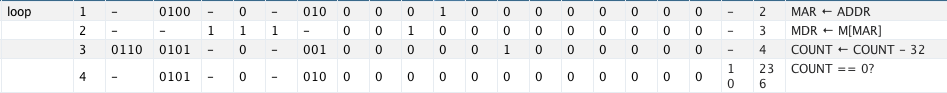
\includegraphics[width=16cm]{listing/row1-4.png}
\leavevmode \\
Zunächst wird die Adresse gesetzt (anfangs 0), der Wert an der Adresse ausgelesen und in \texttt{MDR} abgelegt.
Dies ist der Schleifenkopf und \texttt{ADDR} entspricht der Lauf-Variable.
Wir ziehen 32 vom \texttt{COUNT}-Register ab, welches bereits mit der Anzahl Bits des Benchmarks gefüllt wurde.
Ist \texttt{COUNT} Null, ist das Programm vorbei, wenn nicht, springen wir zum Analyseprogramm.
Im ersten Durchlauf liegt nun im Register \texttt{MDR} die Zahl 16843022.

\leavevmode \\
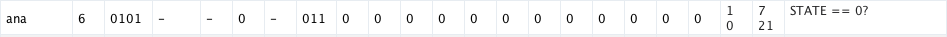
\includegraphics[width=16cm]{listing/row6.png}
\leavevmode \\
Entsprechend des Zustands wird hier unterschieden zwischen Kanalnummer- und Startsequenzsuche. Im ersten Durchlauf
wird natürlich zunächst einmal eine Startsequenz gesucht und der Zustand ist Null (0).

\leavevmode \\
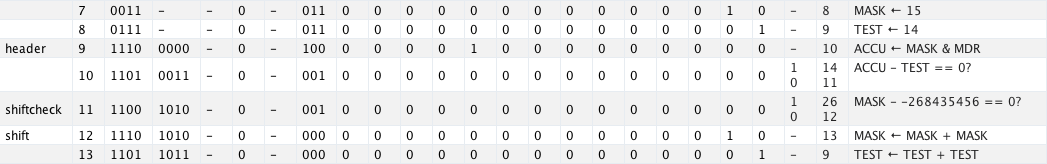
\includegraphics[width=16cm]{listing/row7-13.png}
\leavevmode \\
Zunächst setzen wir die Bitmaske auf 15 und den Subtraktionswert auf 14, dann
wird die Bitmaske auf den Wert aus \texttt{MDR} angewendet und anschließend der Subtraktionswert abgezogen, um
zu überprüfen, ob diese im Wert enthalten ist. Ist dies der Fall, so springen wir zur Zeile mit dem Label \dq new\dq, 
da es sich um ein neues Datenpaket handelt. Wenn die Startsequenz jedoch nicht finden l{\"a}sst suchen wir weiter, indem die Bitmaske (und der Subtraktionswert)
so lange nach links geschiftet (hier: effektiv verdoppelt) werden (Z. 12 und 13) bis das Muster gefunden wurde, oder die Bitmaske den Maximalwert (Z. 11) erreicht hat.
In diesem konkreten Fall wenden wir $16843022 \text{ AND } 15$ an und finden
die Startsequenz.

\leavevmode \\
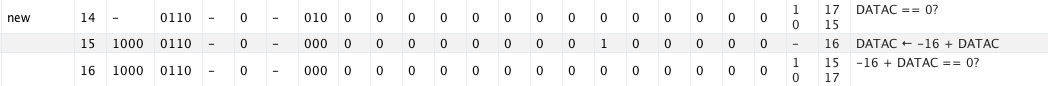
\includegraphics[width=16cm]{listing/row14-16.png}
\leavevmode \\
Hier wird die Datenlänge überprüft, die wir jedoch für den Moment ignorieren können, wir überspringen im ersten Fall auch den Speicheralgorithmus und machen mit Zeile 24 weiter:

\leavevmode \\
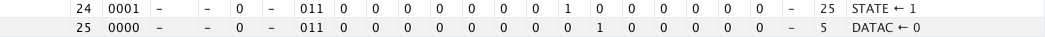
\includegraphics[width=16cm]{listing/row24-25.png}
\leavevmode \\
Da wir die Startsequenz gefunden haben, setzen wir nun den Zustand auf 1 und initialisieren die Datenlänge mit 0. Danach springt
das Programm zurück zur Schleife:

\leavevmode \\
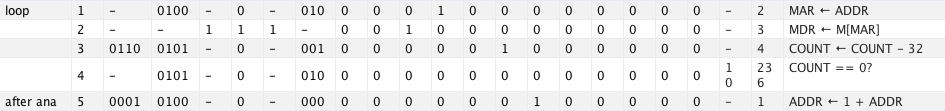
\includegraphics[width=16cm]{listing/row1-5.png}
\leavevmode \\
In Zeile 5 wird die Adresse im Register \texttt{ADDR} inkrementiert und wir springen zum Schleifenkopf zurück, um die nächste
Iteration zu starten. Wir laden nun den Wert 16842760 aus dem Speicher und übergeben ihn dem Analyseprogramm.

\leavevmode \\
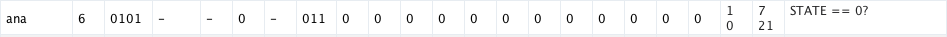
\includegraphics[width=16cm]{listing/row6.png}
\leavevmode \\
Wir überprüfen erneut den Zustand und springen nun zum Auslesen der Kanalnummer (Z. 27), da wir uns in Zustand 1 befinden.

\leavevmode \\
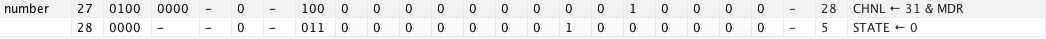
\includegraphics[width=16cm]{listing/row27-28.png}
\leavevmode \\
Mit der Bitmaske 31 lesen wir die Kanalnummer aus der Zahl aus, speichern sie im Register \texttt{CHNL}
und setzen anschließend den Zustand wieder auf 0 und springen zur Schleife
zurück.

\leavevmode \\
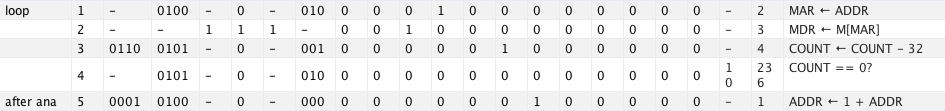
\includegraphics[width=16cm]{listing/row1-5.png}
\leavevmode \\
Nun laden wir den Wert 16843009 aus dem Speicher und übergeben ihn dem Analyseprogramm.

\leavevmode \\
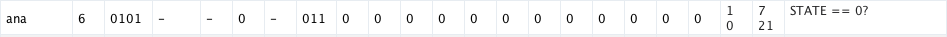
\includegraphics[width=16cm]{listing/row6.png}
\leavevmode \\
Nun sind wir wieder im Zustand 0, suchen also wieder nach der Startsequenz.

\leavevmode \\
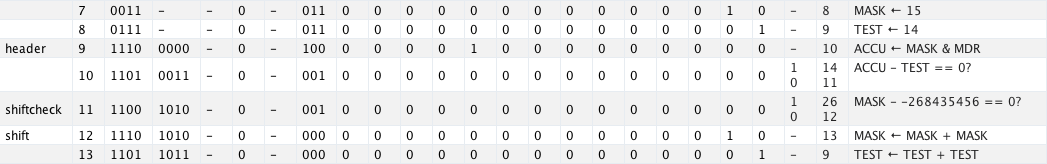
\includegraphics[width=16cm]{listing/row7-13.png}
\leavevmode \\
Die Startsequenz kann nicht gefunden werden, also springen wir zur Zeile 26.

\leavevmode \\
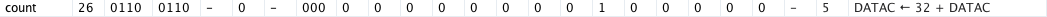
\includegraphics[width=16cm]{listing/row26.png}
\leavevmode \\
Wir addieren die Länge der ausgelassenen Zahl in Bits (32) zur aktuellen Gesamtlänge des Datenfeldes (hier 0) und
springen zurück zur Schleife.

\leavevmode \\
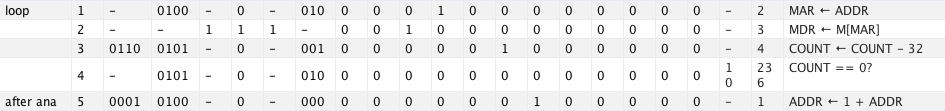
\includegraphics[width=16cm]{listing/row1-5.png}
\leavevmode \\
Wir überspringen für dieses Beispiel Block 4 im Speicher und machen mit Adresse 5 weiter; Wert: 16843022.

\leavevmode \\
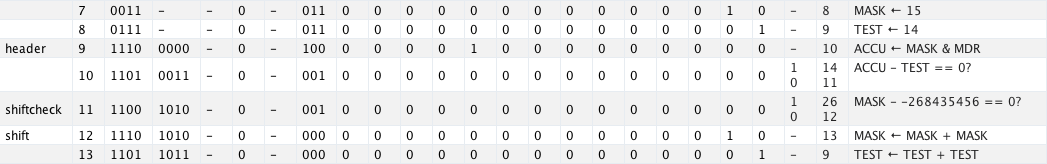
\includegraphics[width=16cm]{listing/row7-13.png}
\leavevmode \\
Wir suchen erneut nach der Startsequenz und finden sie, nun ziehen wir 16 von der gezählten Länge ab (Anzahl Bits des Headers, die wir
mitgezählt haben) und übergeben dem Speicherprogramm:

\leavevmode \\
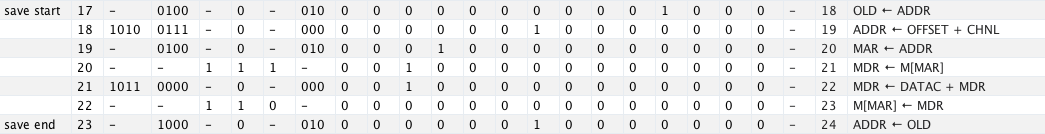
\includegraphics[width=16cm]{listing/row17-23.png}
\leavevmode \\
Zunächst wird die aktuelle Adresse zwischengespeichert, danach addieren wir zu unserem OFFSET die Kanalnummer und benutzen das Ergebnis
als neue Adresse. Dann wird der aktuelle Wert an der Adresse ausgelesen und wir addieren unsere gerade gezählte Länge dazu (Zeile 15).
Anschließend wird der neue Wert im HS abgelegt und wir stellen die ursprüngliche Adresse wieder her.

\leavevmode \\
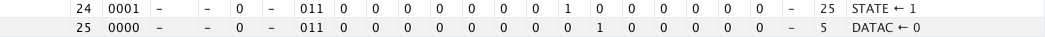
\includegraphics[width=16cm]{listing/row24-25.png}
\leavevmode \\
Nun wird wie zuvor die Datenlänge wieder mit 0 initialisiert, der Zustand auf 1 gesetzt und es wird zurück zur Schleife gesprungen.

\leavevmode \\
Dieser Vorgang wird nun wiederholt, bis das Register \texttt{COUNT} Null ist. Dabei entsteht für dieses Beispiel folgende Tabelle im HS:

\begin{table}[h!]
    \begin{tabular}{l|l}
    Adresse & Wert            \\
    \hline                    \\
    207   & 80       \\
    208   & 0        \\
    ...   & 0        \\
    20E   & 80       \\
    \end{tabular}
\end{table}

\newpage

\section{Verbesserungsvorschläge} 
Wenn man den Algorithmus dieser Maschine verbessert, sollte man immer abw{\"a}gen, ob die Verbesserung der Effizenz des Algorithmus auch eine Verbesserung der Verst{\"a}ndlichkeit mit sich bringt. Denn wenn man davon ausgeht, dass ein anderer Entwickler ein Projekt irgendwann wieder aufgreift und weiter entwickelt, muss man schauen, welche Verbessungen sinnvoll w{\"a}ren. 
Wir haben uns einige Verbesserungen überlegt: 
\begin{enumerate} 
\item Generell könnte man einige Register und Konstanten zusammenfassen bzw. vereinfachen.
\item Die Multiplexer könnten durch etwas Planung gekürzt werden. (z.B. die Register sinnvoller anschließen)
\item Man könnte den Analysealgorithmus noch vereinfachen und ihn noch mehr wie einen Automaten ablaufen lassen.
\item Genaueres Bit-Zählen der Länge der Datenteile
\end{enumerate}

\section{Anhang}

\subsection{Abb. 1: Basismaschine}
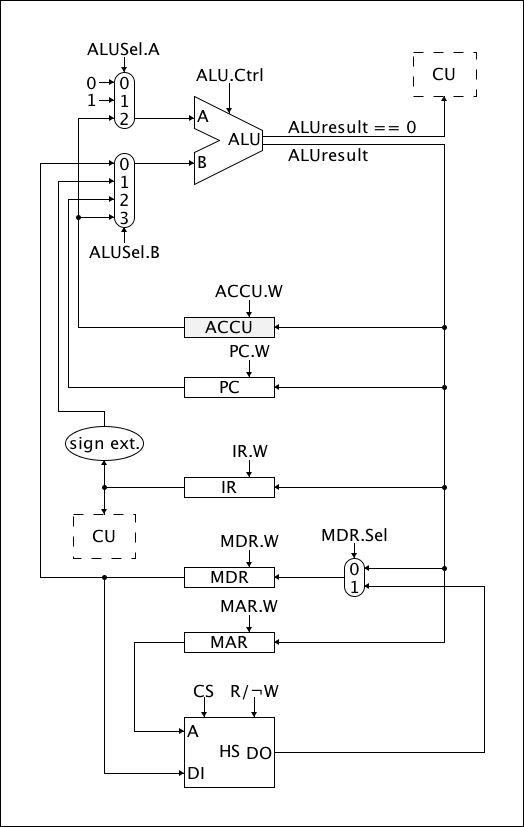
\includegraphics[width=12cm]{schematics.png}

\subsection{Abb. 2: Flussdiagramm des Speicherausleseprogramms}
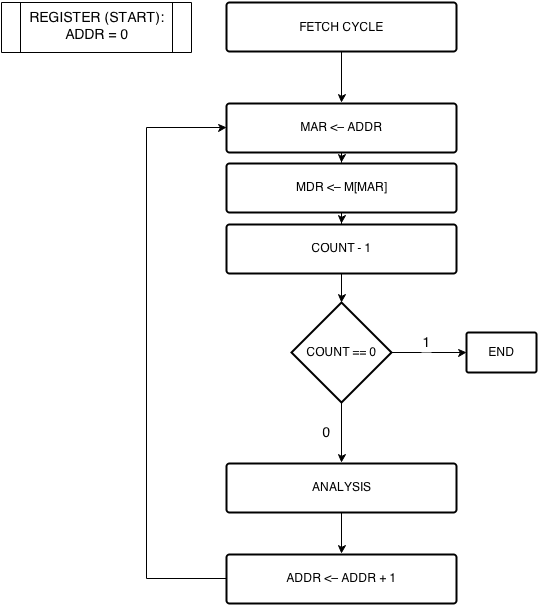
\includegraphics[width=13cm]{readFromMemory.png}

\subsection{Abb. 3: Flussdiagramm des Analyseprogramms}
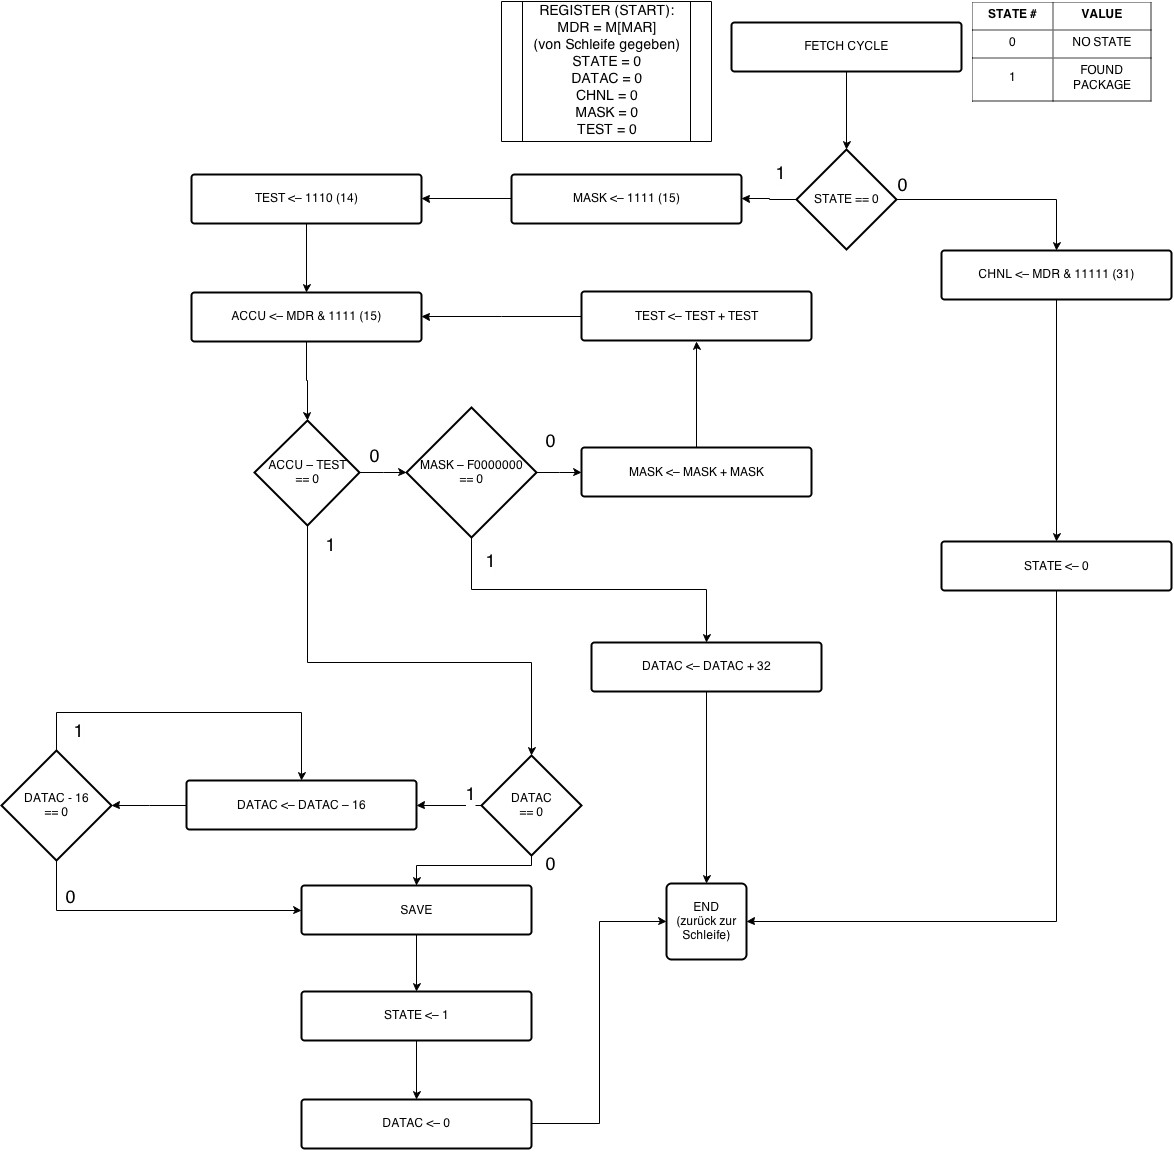
\includegraphics[width=18cm]{analyseData.png}

\subsection{Abb. 4: Flussdiagramm des Speicherprogramms}
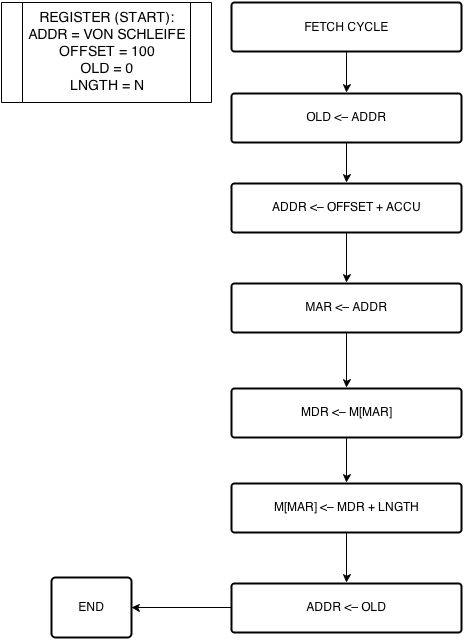
\includegraphics[width=9cm]{saveToHS.png}

\subsection{Abb. 6: Aufbau der erweiterten Maschine}
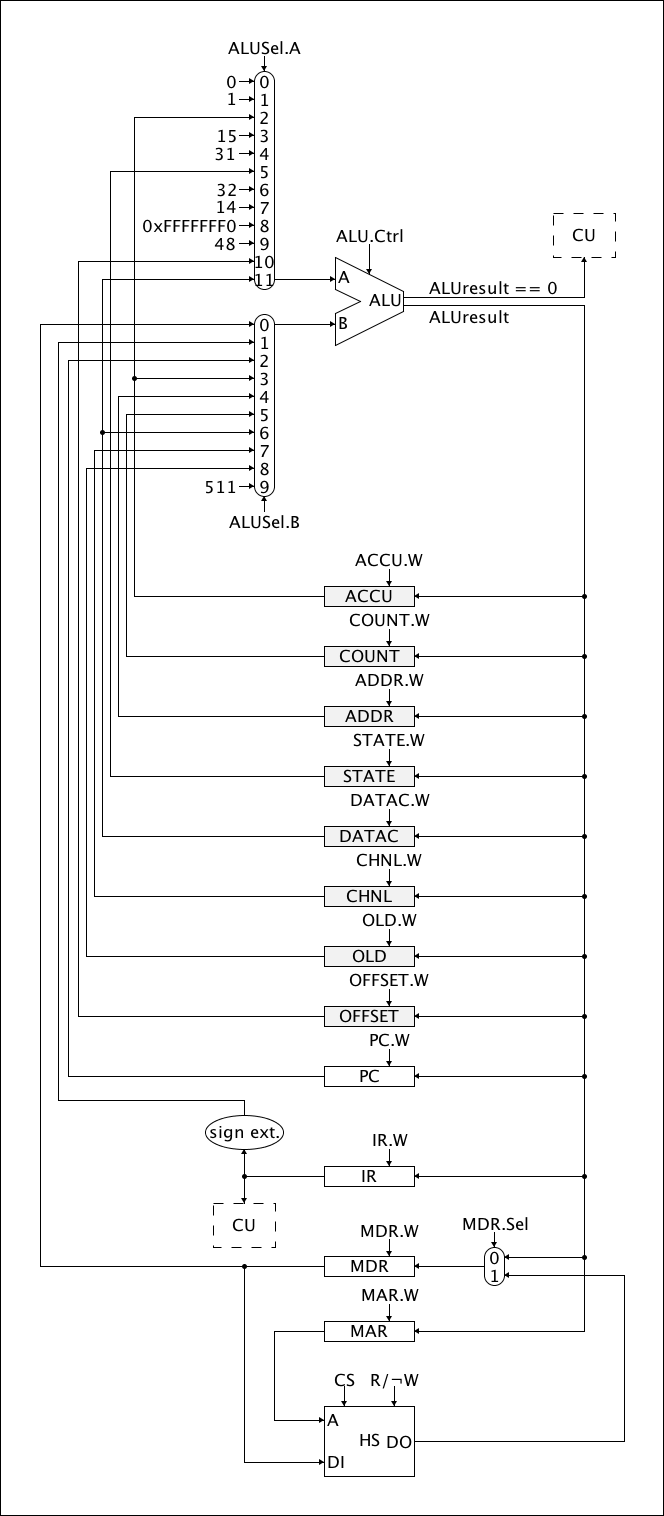
\includegraphics[height=19cm]{schematics_added.png}

\subsection{Abb. 7: Vollständige Steuertabelle}
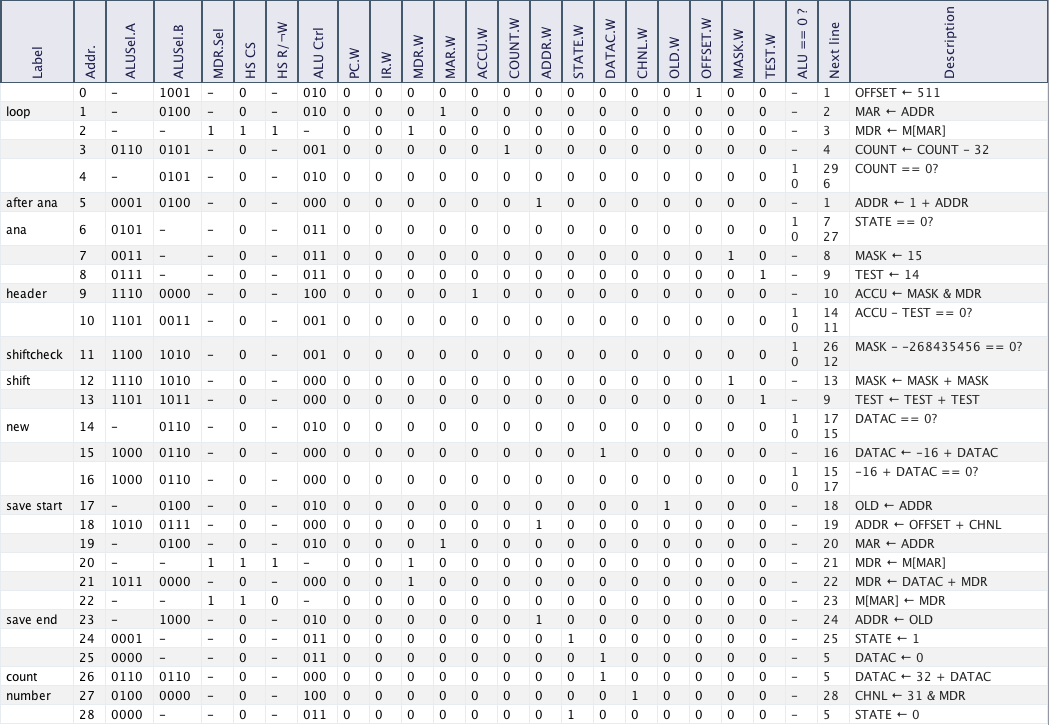
\includegraphics[width=18cm]{signal_table.png}

\newpage



\section{Hilfsmittel}
Wir haben folgende Quellen benutzt:
\begin{enumerate} 
\item Wikipedia: \dq Mask (computing)\dq \\ \string[\url{http://en.wikipedia.org/wiki/Mask_(computing)}\string]
\item Wikipedia: \dq Bitweiser Operator\dq \\ \string[\url{http://de.wikipedia.org/wiki/Bitweiser_Operator}\string]
\item Git VCS zur Quellcodeorganisation und Synchronisation
\item GitHub zur Projektorganisation und Quellcodesynchronisation
\item Flowcharts: \string[\url{https://www.draw.io}]
\item SRA Minimax-Simulator
\item Informationsfolien (Aufgabenstellung)
\item Materialien der Veranstaltung \dq Grundlagen der Rechnerarchitektur\dq von Prof. Dr.-Ing. habil. J{\"u}rgen Brehm
\end{enumerate}

\end{document}
